% Massimo Zannoni - Curriculum Vitae
%
% This work is licensed under a Creative Commons Attribution-ShareAlike 4.0 International License (CC BY-SA 4.0)

\documentclass[a4paper]{article}
\usepackage{graphicx}
\usepackage[top=2.4cm, bottom=2.4cm, left=2cm, right=2cm]{geometry}
\usepackage[utf8]{inputenc}
\usepackage{hyperref}
\usepackage[english]{babel}

%% set the font family
\usepackage[condensed,math]{kurier}
%% set the font encoding
\usepackage[T1]{fontenc}
%% details about the font
%% https://ctan.org/tex-archive/fonts/kurier/

%\usepackage{mdwlist} % needed for itemize*
%\usepackage{tabu} % package for advanced table features
\usepackage{longtable}
\usepackage{array}

\usepackage{enumitem}
%next line to avoid vertical separation before an itemize section
%\setlist{nolistsep}

% Personal details
\def\nome{Massimo Zannoni}
\def\email{myemail@someservice.abc}
\def\telefono{+00 11 22 33 44}
\def\nazionalita{Italian}
\def\datadinascita{00.00.1900}
\def\genere{Male}
\def\indirizzo{Funnystreet, 1 \newline 0000 Zürich \newline CH}

% Define some lengths used in the document
\newlength{\sectsep}
\setlength{\sectsep}{0.6cm}
\newlength{\detsep}
\setlength{\detsep}{0.4cm}

% Edit PDF file properties
\hypersetup{
  pdfauthor = {\nome},
  pdfcreator = {\nome},
  pdfkeywords = {electronics, IC design, RF measurement, optoelectronics, engineering},
  pdftitle = {\nome ~- Curriculum Vitae},
  pdfsubject = {Curriculum Vitae},
  % next line to avoid links from being blue and underlined
  hidelinks
}

% Format two pieces of text, one left aligned and one right aligned
\newcommand{\headerrow}[2]
{\begin{tabular*}{\textwidth}{l@{\extracolsep{\fill}}r}
	#1 &
	#2 \\
\end{tabular*}}

% Make lists with diamonds and compact spacing
\renewenvironment{itemize}{
  \begin{list}{$\diamond$}{
    \setlength{\topsep}{0.25em}
    \setlength{\itemsep}{0em}
    \setlength{\parskip}{0pt}
    \setlength{\parsep}{0em}
  }
}{
  \end{list}
}

% Make lists with small dots and compact spacing
\newenvironment{itemize2}{
  \begin{list}{$\cdot$}{
    \setlength{\topsep}{0.25em}
    \setlength{\itemsep}{0em}
    \setlength{\parskip}{0pt}
    \setlength{\parsep}{0em}
  }
}{
  \end{list}
}

\begin{document}
  \begin{longtable}{r || l}

  % 1st row: Title, details and photo
  \hfill
  & \begin{minipage}{0.5\textwidth}
      \vspace{0.2\sectsep}
      \section*{\nome}
      \vspace{\detsep}
      \indirizzo \vspace{\detsep} \\
      \href{mailto:\email}{\email} ~|~ \telefono \vspace{\detsep} \\
      \datadinascita ~|~ \nazionalita ~|~ \genere \vspace{\detsep} \\
    \end{minipage}
    %\hfill
    \begin{minipage}{0.3\textwidth}
      \vspace{0.4cm}
      {\centering 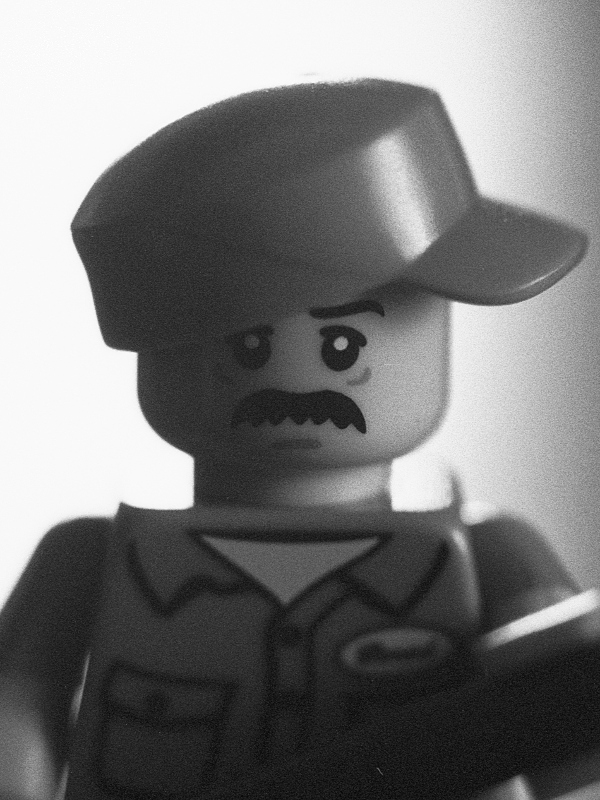
\includegraphics[width=0.5\textwidth]{pics/portrait} \vspace{0.2cm} \\
       %\datadinascita ~||~ \nazionalita  ~||~ \genere \vspace{0.2cm} \\ % put details below the photo
      }
    \end{minipage} \\
  \hline \hline

  %2nd row: Working experience
  & \begin{minipage}{0.9\textwidth}
      \vspace{\sectsep}
      \subsection*{Working Experience}
      \subsubsection*{Design Engineer}
      \headerrow
  		{\textbf{GigOptix-Helix AG} (subsidiary of GigPeak, Inc.)}{\emph{2013 - current}}
      \\
      \headerrow
        {\emph{Seefeldstrasse 45, 8008 Zürich, CH}}{}
      \\
      \headerrow
        {Optoelectronics}{}

      \begin{itemize}
          \item High-speed Analog IC design in BiCMOS technology
          \begin{itemize2}
              \item 28 Gbit/s TIA receivers and VCSEL drivers
          \end{itemize2}
          \item RF and optical measurement
          \item Customer support and RMA analysis
          \item Production support
          \item IT and network infrastructure maintenance
      \end{itemize}

      \subsubsection*{Thesis Worker}
      \headerrow
  		{\textbf{ABB AB Corporate Research Center}}{\emph{July 2012 - December 2012}}
      \\
      \headerrow
        {\emph{Forskargränd 7, 722 26 Västerås, Sweden}}{}
      \\
      \headerrow
          {Power Technology Dept., Electric Power System Group}{}

      \begin{itemize}
          \item Semiconductor device modeling
          \item Power Electronics
      \end{itemize}

    %   \subsubsection*{Worker}
    %   \headerrow
 %  		{\textbf{Rodolfi Mansueto Spa}}{\emph{2004 - 2011}}
    %   \\
    %   \headerrow
    %     {\emph{Strada Qualatico 14, 43044 Ozzano Taro, PR, Italy}}{\emph{(2 months every summer)}}
    %   \\
    %   \headerrow
    %       {Food processing}{}
    %
    % %   \begin{itemize}
    % %       \item Responsible for a sterilization plant
    % %   \end{itemize}
  \end{minipage} \\[\sectsep]

  %3th row: Education
  & \begin{minipage}{0.9\textwidth}
      \vspace{\sectsep}
      \subsection*{Education}
      \subsubsection*{MSc in Electronic Engineering}
      \headerrow
  		{\textbf{Università degli Studi di Parma, Italy}}{\emph{2009 - 2013}}
      \\
      \headerrow
        {\emph{Faculty of Engineering}}{}
      \\
      \headerrow
        {Analog/Digital IC Design, Semiconductor Physics, Sensor Technology, Power Electronics}{}

      \begin{itemize}
          \item Thesis: \emph{PSpice Modeling of 4.5 kV StakPak\textsuperscript{TM} Modules}
          \item Grade: 107/110
      \end{itemize}

      \subsubsection*{BSc in Electronic Engineering}
      \headerrow
  		{\textbf{Università degli Studi di Parma, Italy}}{\emph{2005 - 2009}}
      \\
      \headerrow
        {\emph{Faculty of Engineering}}{}
      \\
      \headerrow
        {Electronics, Electrotechnics, Information Technology, Controls, PCB Design}{}

      \begin{itemize}
          \item Thesis: \emph{Experimental Characterization of a Magneto-hydrodynamic Micro-Stirrer}
          \item Grade: 108/110
      \end{itemize}
      \vfill
  \end{minipage} \\

  %4th row: Other skills and competences
  & \begin{minipage}{0.9\textwidth}
      \vspace{0.2\sectsep}
      \subsection*{Personal Skills and Competences}
      \subsubsection*{Languages}
      \begin{tabular}{rl}
        \textbf{Italian:}&Native\\
        \textbf{English:}&Fluent\\
        \textbf{German:}&Beginner/Intermediate\\
      \end{tabular} \vspace{1.5ex} \\
      \hspace*{0.5em} {\footnotesize \emph{See Common European Framework (CEF) self-assessment table in the appendix.}}

      \subsubsection*{Technical Skills and Competences}
      \begin{itemize}
          \item Analog IC Design
          \item Full-custom analog IC layout
          \item RF and optical measurements
          \item Relate models to physical reality
          \item Attitude to solve practical problems where limited standardization exists
          \item Data analysis and elaboration
          \item Frequently switch between different kinds of task
          \item Clearly describe design issues before organization employees
          \item Hand-working: good familiarity with tools and instruments for building electronic systems; basic skills in the use of main mechanic hand and power tools
      \end{itemize}

      \subsubsection*{Computer Skills and Competences}
      \begin{tabular*}{\textwidth}{r p{0.75\textwidth}}
        Operating Systems:&{Linux: very good knowledge\newline Microsoft Windows: good knowledge}\\[0.5ex]
        Electronic CAD:&Cadence DFII (Virtuoso, Spectre), SPICE, Cadence OrCAD (PSpice), Cadence SoC Encounter, Agilent ADS\\[0.5ex]
        Programming:&Python, C/C++, Matlab/Octave, shell scripting, VHDL, Verilog/VerilogA, {\fontfamily{cmr}\selectfont\LaTeX}\\[0.5ex]
        Version Control:&Subversion, ClioSoft SOS
      \end{tabular*}\\

      \subsubsection*{Organizational and Social Competences}
      \begin{itemize}
          \item 2009-2012: responsible for design and realization of the electrical system of the racing car in the \emph{Formula SAE} (Formula Student) team of the University of Parma
          \item 4 years experience as executive in a volleyball sport association
          \item Occasional collaboration with a cooperative, named \emph{Lune Nuove}, in Parma, organizing cultural events, as assistant in logistics
          \item Volleyball player for 12 years, then Ultimate Frisbee player until present day
          \item Teaching and organizing experience in a course of basic computer ability
      \end{itemize}
      \subsubsection*{Other Skills and Competences}
      \begin{itemize}
          \item Good photo-editing and computer drawing skills
          \item Basic sound engineering skills
          \item Swiss Driving License: Category A and B
      \end{itemize}

      \subsubsection*{Personal Interests}
      \begin{itemize}
          \item Love for traveling
          \item Photography
          \item Guitar player (formerly in an amateur rock band)
      \end{itemize}

      \subsubsection*{Annexes}
      \begin{itemize}
          \item Appendix including publications, references and main projects developed during studies
          \item Reference letter by former manager available upon request
      \end{itemize}
      \vfill
    \end{minipage} \\

  \end{longtable}
\end{document}
